\documentclass{article}
\usepackage{arxiv}
\setcounter{secnumdepth}{2} 
\fancyfoot{}
\sloppy
\usepackage{wrapfig}
\usepackage{booktabs} % For formal tables
\usepackage{caption}
\usepackage{subcaption}
\usepackage{amsmath,amssymb,amsfonts}
\usepackage{algorithmic}
\usepackage[numbers]{natbib}
\usepackage{comment}
\usepackage[linesnumbered,ruled,vlined]{algorithm2e}
\SetKwComment{Comment}{$\triangleright$\ }{}
\usepackage{graphicx}
\usepackage{textcomp}
\usepackage{multirow}
\usepackage{hyperref}
\usepackage[table, svgnames, dvipsnames]{xcolor}
\usepackage{makecell, cellspace, caption}
\def\BibTeX{{\rm B\kern-.05em{\sc i\kern-.025em b}\kern-.08em
    T\kern-.1667em\lower.7ex\hbox{E}\kern-.125emX}}

\def\A{{\bf A}}
\def\a{{\bf a}}
\def\B{{\bf B}}
\def\b{{\bf b}}
\def\C{{\bf C}}
\def\c{{\bf c}}
\def\D{{\bf D}}
\def\d{{\bf d}}
\def\E{{\bf E}}
\def\e{{\bf e}}
\def\F{{\bf F}}
\def\f{{\bf f}}
\def\g{{\bf g}}
\def\h{{\bf h}}
\def\G{{\bf G}}
\def\H{{\bf H}}
\def\I{{\bf I}}
\def\K{{\bf K}}
\def\k{{\bf k}}
\def\l{{\bf l}}
\def\M{{\bf M}}
\def\m{{\bf m}}
\def\N{{\bf N}}
\def\n{{\bf n}}
\def\Q{{\bf Q}}
\def\q{{\bf q}}
\def\R{{\bf R}}
\def\S{{\bf S}}
\def\s{{\bf s}}
\def\T{{\bf T}}
\def\U{{\bf U}}
\def\u{{\bf u}}
\def\V{{\bf V}}
\def\v{{\bf v}}
\def\W{{\bf W}}
\def\w{{\bf w}}
\def\X{{\bf X}}
\def\x{{\bf x}}
\def\Y{{\bf Y}}
\def\y{{\bf y}}
\def\Z{{\bf Z}}
\def\z{{\bf z}}
\def\0{{\bf 0}}
\def\1{{\bf 1}}
\def\RB{{\mathbb R}}

\newcommand{\red}[1]{{\color{red}#1}}

\title{Study Note on Paligemma} % \\

\author{
% suggested author list, if you work with another student, provide names and email addresses for both.
Linsen Li\\
Computer Science in Tulane\\
lli23@tulane.edu
}
\date{\today}
\begin{document}
\maketitle
\begin{abstract}
This article is to log the implementation of Paligemma\cite{beyer2024paligemma}. 
\end{abstract}

% Include the sections you need to present
\section{Introduction}
PaliGemma\cite{beyer2024paligemma} is a model that excels at interpreting and understanding both images and text. 
It's used for tasks like generating descriptions of images, answering questions based on visual content, 
and analyzing complex visuals like infographics and satellite images. The input to PaliGemma can be an 
image, text, or both, and the output might be a text description, an answer to a question, or information derived 
from the image. It's designed to handle a wide range of vision-language tasks efficiently, 
even though it is smaller in size compared to some other advanced models.

The architecture of PaliGemma-3B, as shown in Figure~\ref{fig:paligemma}, is inspired by the PaLI-3 model and combines the SigLIP visual encoder with the 
Gemma 2B language model. When PaliGemma-3B processes input, images are first converted into "soft tokens" by the SigLIP encoder. 
Simultaneously, any accompanying text, referred to as the "prefix," is tokenized by Gemma's tokenizer. 
These image tokens and text tokens are then combined and fed into the Gemma decoder, which uses full block-attention to generate 
the final output text, or "suffix," in an auto-regressive manner. 

\begin{figure}[htbp]
    \centering
    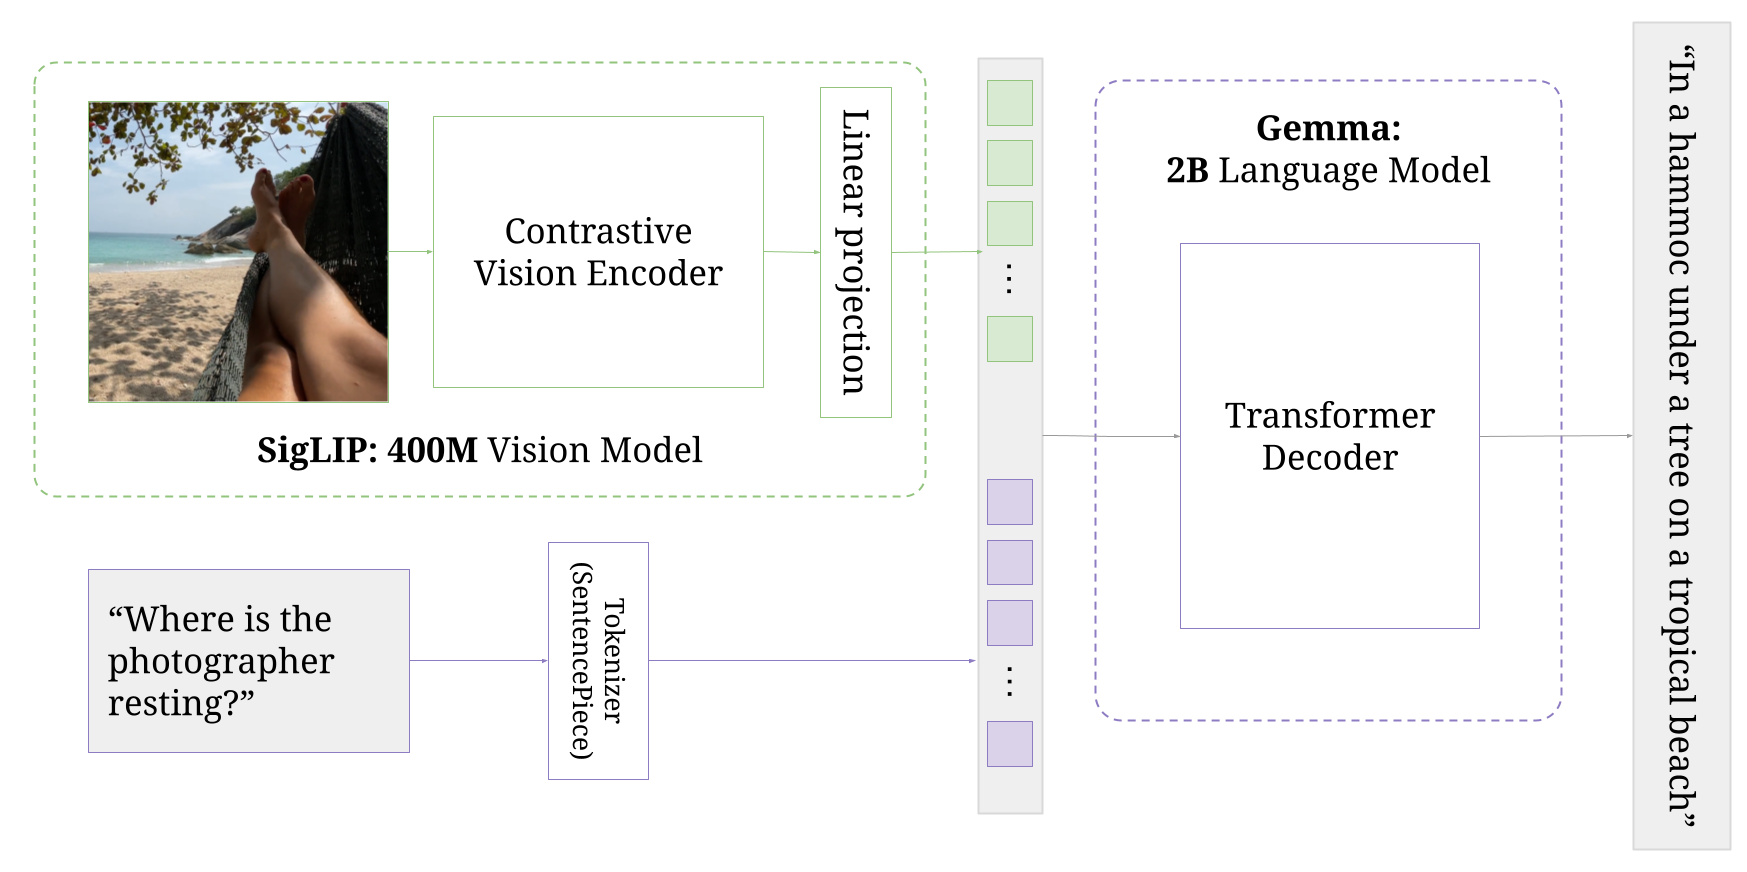
\includegraphics[width=0.8\textwidth]{figures/paligemma.png}
    \caption{Architecture f Paligemma.}
    \label{fig:paligemma}
\end{figure}


\section{Related Work}
Describe background. Introduce and cite what other people have done for this topic. Discuss the limitations of current approaches.

\section{SigLIP}
Paligemma uses the SigLIP model\cite{zhai2023sigmoid} as their Contrasive Vision Encoder. 



\section{Experimental Setup}
Describe how you setup the experiments and the questions you try to answer using the experiments.
\subsection{Data}
Describe datasets you use including where you get the data, data statistics, etc. We encourage you to use public datasets.
\subsection{Evaluation Metrics}
Introduce evaluation metrics you use; If necessary, use equations.
\subsection{Comparison Methods}
List other methods you compare with (with citations) and the reasons you choose them.

\section{Results}
Analyze the results you get. Use tables or figures to show the results.
\begin{footnotesize}
\bibliographystyle{plainnat}
\bibliography{reference}
\end{footnotesize}%
\end{document}
